\documentclass[12pt]{article}
\usepackage{preamble}
\usepackage{longtable}

\geometry{a4paper, left=2.5cm, right=2.5cm, top=2cm, bottom=2.5cm}

\pagestyle{plain}

\newcommand{\placeholder}[1]{{\color{magenta}#1}}

\chead{
    \begin{minipage}{1\linewidth}
        \begin{wrapfigure}{r}{0pt}
            \includegraphics[height=1cm]{images/logo}
        \end{wrapfigure}
        {
            \centering
            \sffamily\scriptsize
            \textbf{
                Санкт-Петербургский национальный исследовательский университет \\
                информационных технологий, механики и оптики}
            %th3p4g
            \vspace{2mm}

            \quad\quad\quad\quad\quad\quad\ \textbf{УЧЕБНЫЙ ЦЕНТР ОБЩЕЙ ФИЗИКИ ФТФ}
        }
    \end{minipage}
}



\begin{document}
    \vspace*{2\baselineskip}

    \thispagestyle{fancy}

    \noindent
    \textbf{Группа} \underline{M3200\hspace{4.5cm}} \hfill \textbf{К работе допущен} \underline{\hspace{4cm}} \\[0.5cm]
    \textbf{Студенты} \underline{Комашко А., Семёнов Д.\hspace{0.45cm}} \hfill \textbf{Работа выполнена} \underline{\hspace{4cm}} \\[0.5cm]
    \textbf{Преподаватель} \underline{Хвастунов Н. Н.\hspace{0.95cm}} \hfill \textbf{Отчет принят} \underline{\hspace{4.85cm}} \\


    \begin{center}
    {\huge \textbf{Рабочий протокол и отчёт по\\ лабораторной работе №3.02}}

        \smallvspace

        {\Large Характеристики источника тока}
    \end{center}


    \noindent
    1. \textbf{Цель работы.}

    \begin{enumerate}
        \item Исследовать зависимость полной мощности, полезной мощности,
        мощности потерь, падения напряжения во внешней цепи и КПД
        источника от силы тока в цепи.
        
        \item Найти значения параметров источника: электродвижущей силы и
        внутреннего сопротивления, оценить их погрешность.
    \end{enumerate}

    \mediumvspace

    \noindent
    2. \textbf{Задачи, решаемые при выполнении работы.}

    \begin{enumerate}
        \item Получение данных при помощи измерений (построение экспериментальной выборки)
        \item Анализ полученных результатов - исследование зависимостей физических величин от силы тока в цепи
        \item Нахождение параметров источника тока
    \end{enumerate}

    \mediumvspace

    \noindent
    3. \textbf{Объект исследования} \\
    Цепь, собранная на стенде СЗ-ЭМ01. Контур с исследуемым источником тока и регулируемым внешним сопротивлением.


    \mediumvspace

    \noindent
    4. \textbf{Метод экспериментального исследования.} \\
    Прямые измерения значений силы тока и напряжения на участке цепи

    \newpage

    \noindent
    5. \textbf{Рабочие формулы и исходные данные.}

    \text{Закон Ома для замкнутой цепи}
\[
I = \frac{\mathcal{E}}{R + r}
\]

\text{Где:}
\begin{center}
    $I - \text{сила тока}$ \\
    $\mathcal{E} - \text{электродвижущая сила (ЭДС)}$ \\
    $r - \text{внутреннее сопротивление источника тока}$ \\
    $R - \text{сопротивление внешней цепи}$
\end{center}

\vspace{0.1cm}

\text{Внутреннее сопротивление источника тока по МНК}
\[
r = \frac{\sum\limits_{i=1}^{n}(I_i - \overline{I})(U_i - \overline{U}))}{\sum\limits_{i=1}^{n}(I_i - \overline{I})^2}
\]

\vspace{0.1cm}

\text{ЭДС на основе известного значения внутреннего сопротивления источника}
\[
\mathcal{E} = \overline{U} + \overline{I}|r|
\]

\vspace{0.1cm}

\text{Полная мощность, развиваемая источником}
\[
P = I\mathcal{E}
\]

\text{Полезная мощность, развиваемая источником во внешней цепи}
\[
P_{R} = I^2R
\]\

\text{Мощность потерь внутри источника}
\[
P_{S} = I^2r
\]

\text{Где:}
\[
P = P_{R} + P_{S}
\]

\vspace{0.1cm}

\text{Коэффициент полезного действия}
\[
\eta = \frac{P_{R}}{P} = \frac{U}{\mathcal{E}} = \frac{\mathcal{E} - Ir}{\mathcal{E}} = 1 - \frac{Ir}{\mathcal{E}}
\]

\vspace{0.1cm}

\text{Абсолютная погрешность с учётом погрешности приборов}
\[
\Delta x = \sqrt{\left(\overline{\Delta x}\right)^2 + \left(\frac{2}{3} \Delta_{\text{и}x}\right)^2}
\]

\text{Где:}
\begin{center}
    $\Delta_{ux} - \text{погрешность прибора}$ \\
    $\Delta x - \text{случайная погрешность (доверительный интервал)}$
\end{center}

\vspace{0.1cm}

\text{Погрешность косвенного значения}
\[
\Delta z = \sqrt{\left(\frac{\partial z}{\partial x_1} \Delta x_1\right)^2 + \left(\frac{\partial z}{\partial x_2} \Delta x_2\right)^2}, \quad z = f(x_1, x_2)
\]

\vspace{0.1cm}

\text{Относительная погрешность}
\[
\varepsilon_x = \frac{\Delta x}{\overline{x}} \cdot 100\%
\]

\vspace{0.1cm}

\text{Абсолютные погрешности для МНК значений внутреннего сопротивления и ЭДС}
\begin{center}
    $\Delta r = 2 \cdot \sqrt{\frac{\sum\limits_{i=1}^N d_i^2}{D (n-2)}}$ \\
    $\Delta \mathcal{E} = 2 \cdot \sqrt{\frac{\sum\limits_{i=1}^N d_i^2}{D (n-2)}\cdot \left(\frac{1}{n} + \frac{\overline{I}^2}{D}\right)}$
\end{center}

\text{Где:}
\[
d_i = U_i - (\mathcal{E} - I_i|r|) \quad \quad D = \sum\limits_{i=1}^N (I_i - \overline{I})^2
\]

    \mediumvspace

    \noindent
    6. \textbf{Измерительные приборы.}

    \smallvspace

    \begin{center}
    \begin{tabular}{|c|m{4cm}|C{2cm}|C{3cm}|c|}
        \hline
        № п/п & Наименование            & Предел\newlineизмерений & Цена деления    & $\Delta_{\text{и}}$ \\
        \hline
        1     & Амперметр               & 20 мА                   & 0.01 \text{мА/дел}                     & 0.01 \text{мА}     \\
        \hline
        2     & Вольтметр               & 20 В                    & 0.01 \text{В/дел}                      & 0.01 \text{В}      \\
        \hline

    \end{tabular}

    \smallvspace

    \textit{Таблица 1.} Измерительные приборы
\end{center}

    \mediumvspace

    \noindent
    7. \textbf{Схема установки. (перечень схем, которые составляют Приложение 1).}

    \hyperlink{schema1}{Схема установки} прилагается в Приложении 1

    \mediumvspace

    \noindent
    8. \textbf{Результаты прямых измерений и их обработки (таблицы, примеры расчетов).}

    \begin{itemize}
    \item Прилагается \hyperlink{table2}{Таблица 2} в Приложении 2
\end{itemize}

\text{Внутреннее сопротивление источника тока по МНК:} \\
    
    $r = \frac{\sum\limits_{i=1}^{n}(I_i - \overline{I})(U_i - \overline{U})}{\sum\limits_{i=1}^{n}(I_i - \overline{I})^2} = -0.67635 \ \frac{\text{В}}{\text{мА}}$

    \smallvspace

    \text{ЭДС источника по МНК:} \\
    
    $\mathcal{E} = \overline{U} + \overline{I}|r| = 10.55377 \ \text{В}$

    \newpage

    \text{Значение тока, при котором достигается максимум значения полезной мощности:}

    $I^* = 7.51 \ \text{мА  - по графику } P_R = P_R(I)$

    $I^* = 7.80 \ \text{мА  - по графику } \eta = \eta(I)$

    \smallvspace

    \text{Максимальная полезная мощность:}

    $P_{R max} = 41.1548 \ \text{мВт - по графику } P_R = P_R(I)$

    \smallvspace

    \text{Сопротивление, соответствующее режиму согласования нагрузки и источника}

    $R_{\text{согл}} = \frac{P_{R max}}{(I^*)^2} = 0.7297 \ \frac{\text{В}}{\text{мА}}$

    \mediumvspace

    \noindent
    9. \textbf{Расчет результатов косвенных измерений (таблицы, примеры расчетов).}

    \text{Расчет абсолютных погрешностей для значений внутреннего сопротивления и ЭДС:}

\begin{center}
    $\sum\limits_{i=1}^{n}d_i^2 = 1.08481 \cdot 10^{-4} \ \text{мА}^2$ \\
    $D = 120,47864 \ \text{мA}^2$ \\
    $\Delta r = 2 \cdot \sqrt{\frac{\sum\limits_{i=1}^N d_i^2}{D (n-2)}} = 1,38526 \cdot 10^{-7} \ \frac{\text{В}}{мА}$ \\
    $\Delta \mathcal{E} = 2 \cdot \sqrt{\frac{\sum\limits_{i=1}^N d_i^2}{D (n-2)}\cdot \left(\frac{1}{n} + \frac{\overline{I}^2}{D}\right)} = 9,60114 \cdot 10^{-6} \ \text{В}$
\end{center}

\text{Расчет относительных погрешностей для значений внутреннего сопротивления и ЭДС:}

\begin{center}
    $\varepsilon_r = \frac{\Delta r}{\overline{r}} \cdot 100\% = 2.048 \cdot 10^{-5}\%$ \\
    $\varepsilon_{\mathcal{E}} = \frac{\Delta \mathcal{E}}{\overline{\mathcal{E}}} \cdot 100\% = 4.549 \cdot 10^{-5}\%$
\end{center}

    \mediumvspace

    \noindent
    10. \textbf{Графики (перечень графиков, которые составляют Приложение 3).}

    \hyperlink{diagram1}{График 1} прилагаются в Приложении 3

    \mediumvspace

    \noindent
    11. \textbf{Окончательные результаты.}

    \text{Доверительный интервал для значения внутреннего сопротивления:}
\[
r = (6.7635000 \pm 0.0000014) \cdot 10^{-1} \ \frac{\text{В}}{\text{мА}} \quad \varepsilon_r = 2.0148 \cdot 10^{-5} \%
\]

\text{Доверительный интервал для значения ЭДС источника:}
\[
\mathscr{E} = (10.553770 \pm 0.000010) \ \text{В} \quad \varepsilon_\mathscr{E} = 4.549 \cdot 10^{-5} \%
\]

\text{Значение тока, при котором достигается максимум значения полезной мощности:}
\[
I^* = 7.51 \ \text{мА} \quad P_{R_\text{max}} = 41.15 \ \text{мВт}
\]

\text{Режим согласования:}
\[
R_{\text{согл}} = 0.73 \ \frac{\text{В}}{\text{мА}} \approx r
\]

\text{Проверка значения силы тока при КПД = 0.5}:
\[
I_{\eta = 0.5}^* = 7.80 \ \text{мА} \quad \Delta I^* = |I^* - I_{\eta = 0.5}^*| = 0.29 \ \text{мА}
\]

    \mediumvspace

    \noindent
    12. \textbf{Выводы и анализ результатов работы.}

    После проведения эксперимента была сформирована выборка, на основе которой были 
вычислены необходимые косвенные параметры мощностей: полезной, потерь и полной, 
а также коэффициент полезного действия (КПД) источника. Были построены графики, 
показывающие зависимости мощностей и КПД от силы тока в цепи. 
С использованием метода наименьших квадратов были определены значения электродвижущей силы (ЭДС) и внутреннего сопротивления, 
а также их погрешности. После расчёта силы тока, при которой достигается максимальная полезная мощность, 
было подтверждено, что в этом случае КПД источника составляет примерно 50\%. 
Также было найдено значение сопротивления, при котором происходит согласование с источником тока, 
и установлено, что оно практически совпадает с внутренним сопротивлением источника.

    \clearpage

    \begin{center}
        \LARGE
        \textbf{Приложение 1. Схема установки}
    \end{center}

    \mediumvspace

    \input{schema1}

    \clearpage

    \begin{center}
        \LARGE
        \textbf{Приложение 2. Таблицы измерений и расчётов}
    \end{center}

    \mediumvspace

    \begin{center}
    \hypertarget{table2}{}

    \renewcommand{\arraystretch}{1.6}

    \begin{tabular}{|c|C{2cm}|C{2cm}|C{2cm}|C{2cm}|C{2cm}|C{2cm}|}
        \hline
        №  & $U$, В & $I$, мА & $P_R$, мВт & $P_S$, мВт & $P$, мВт & $\eta$ \\
        \hline
        1 & 0,9 & 14,27 & 12,843 & 137,726 & 150,602 & 0,0853 \\
        \hline
        2 & 2,08 & 12,53 & 26,062 & 106,187 & 132,239 & 0,1971 \\
        \hline
        3 & 3,16 & 10,93 & 34,539 & 80,800 & 115,353 & 0,2994 \\
        \hline
        4 & 3,9 & 9,84 & 38,376 & 65,488 & 103,849 & 0,3695 \\
        \hline
        5 & 4,52 & 8,92 & 40,318 & 53,814 & 94,140 & 0,4283 \\
        \hline
        6 & 5,1 & 8,06 & 41,106 & 43,938 & 85,063 & 0,4832 \\
        \hline
        7 & 5,48 & 7,51 & 41,155 & 38,146 & 79,259 & 0,5192 \\
        \hline
        8 & 5,83 & 6,99 & 40,752 & 33,046 & 73,771 & 0,5524 \\
        \hline
        9 & 6,15 & 6,51 & 40,037 & 28,664 & 68,705 & 0,5827 \\
        \hline
        10 & 6,45 & 6,07 & 39,152 & 24,920 & 64,061 & 0,6112 \\
        \hline
        11 & 6,68 & 5,73 & 38,276 & 22,206 & 60,473 & 0,6329 \\
        \hline
        12 & 6,89 & 5,42 & 37,344 & 19,869 & 57,201 & 0,6528 \\
        \hline
        13 & 7,13 & 5,06 & 36,078 & 17,317 & 53,402 & 0,6756 \\
        \hline
        14 & 7,33 & 4,76 & 34,891 & 15,324 & 50,236 & 0,6945 \\
        \hline
        15 & 7,29 & 4,82 & 35,138 & 15,713 & 50,869 & 0,6907 \\
        \hline
    \end{tabular}

    \smallvspace

    \textit{Таблица 2.} Результаты прямых измерений и их обработка
\end{center}

    % \input{table3}

    \clearpage

    \begin{center}
        \LARGE
        \textbf{Приложение 3. Графики}
    \end{center}

    \mediumvspace

    \hypertarget{diagram1}{}

\begin{center}
    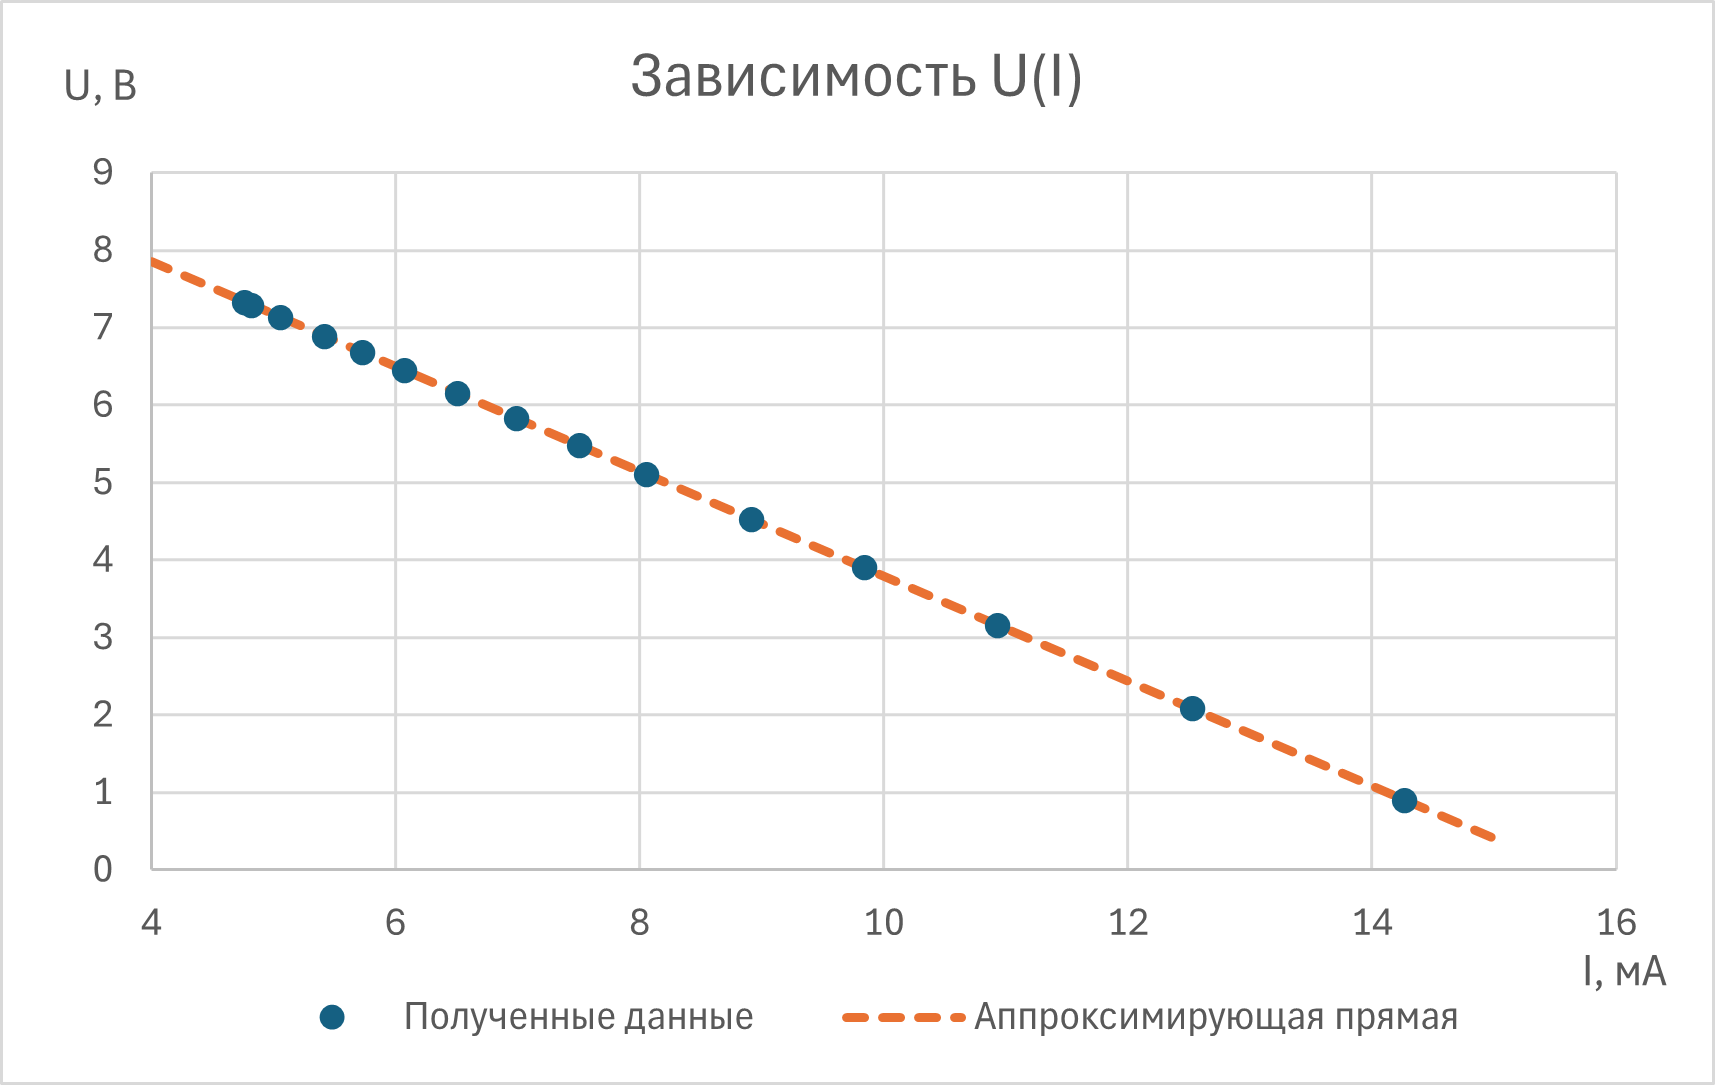
\includegraphics[width=15cm]{images/3.02.1.png}

    \smallvspace

    \textit{График 1.} Зависимость $U(I) = \mathscr{E} - Ir$
\end{center}

\begin{center}
    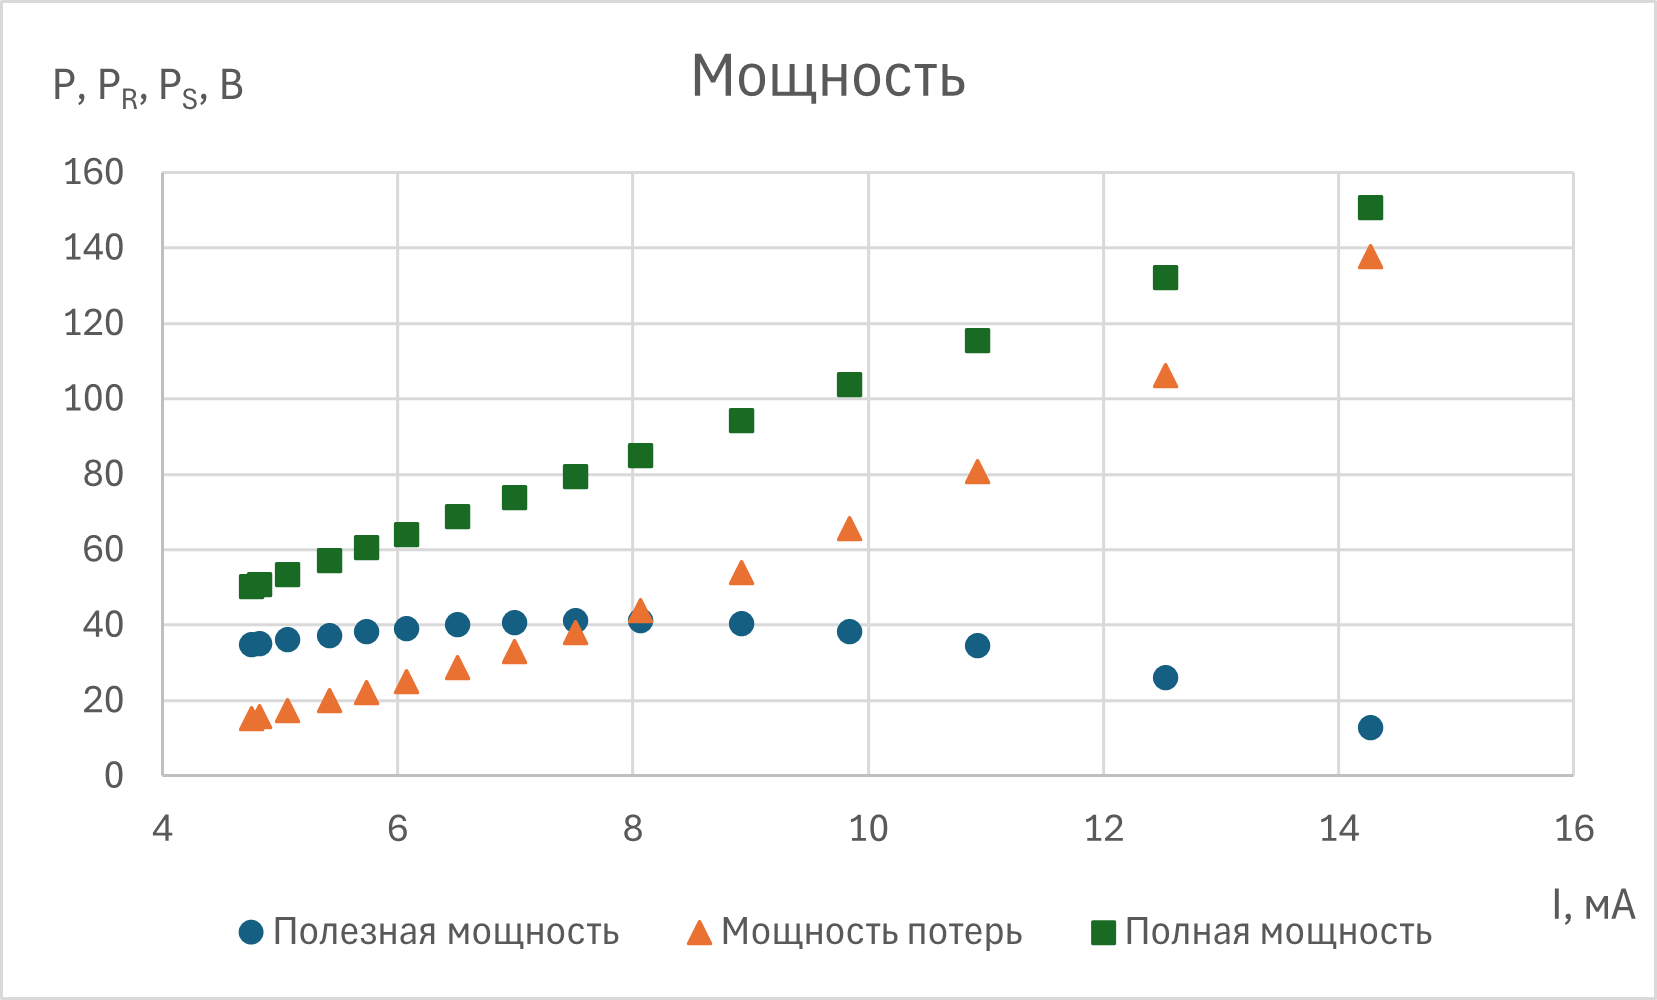
\includegraphics[width=15cm]{images/3.02.2.png}

    \smallvspace

    \textit{График 2.} Мощности $P, P_R, P_S$
\end{center}

\begin{center}
    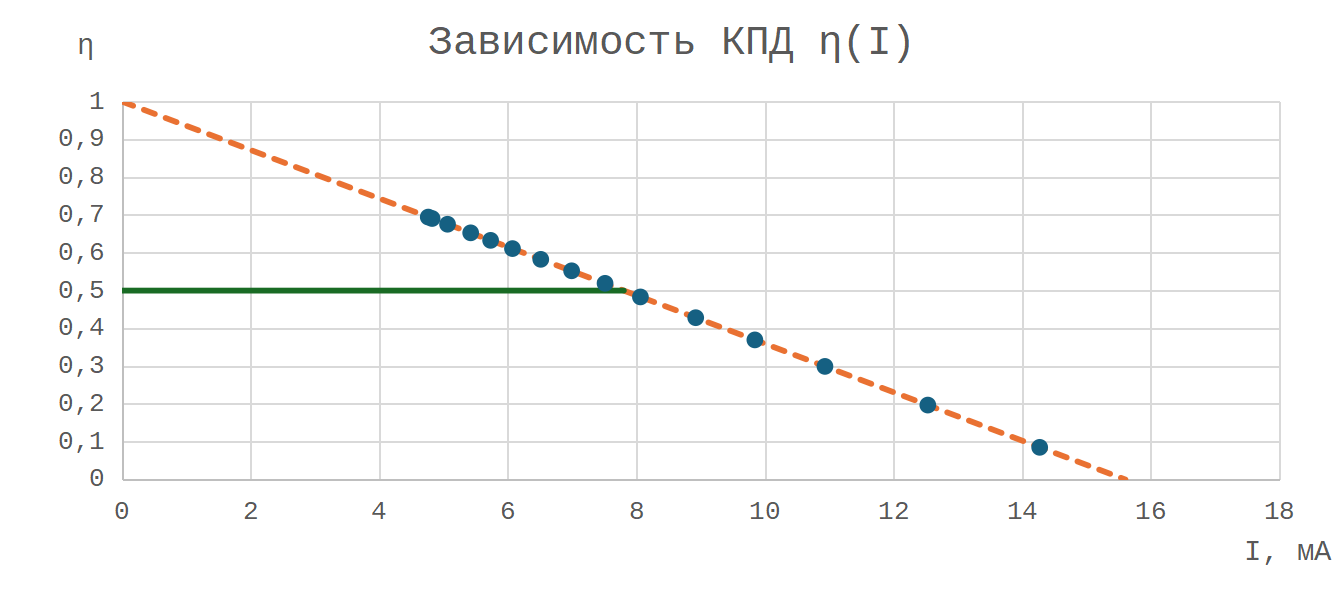
\includegraphics[width=15cm]{images/3.02.3.png}

    \smallvspace

    \textit{График 3.} Зависимость КПД $\eta = \frac{P_R}{P}$
\end{center}



\end{document}